% answers.tex —— 2023 年·全国甲卷·理科 · 参考答案与详细解析片段
% 由 tools/generate_projects.py 依来源总账自 2023/2023_数学真题_全国甲理_试题.md + 2023/2023_数学真题_全国甲理_解析正文.md + 2023/2023_数学真题_全国甲理_答案要点.md 生成，勿手改（改源 MD 后重跑）

\begin{gknotice}
\textbf{解析归属}：下列答案与推导由本库依据固定原卷独立完成，\textbf{不是官方答案}，未引用或声称代表官方发布版本，并经另一角色逐题盲核。

\textbf{题目分节说明}：题面保留 PDF 实际印出的分节文字；第 22、23 题均列出解答，索引题型按本批沿用的 2023 结构登记，不向原题补写作答说明。
\end{gknotice}

\gkanswer{答案速查}

\begin{center}
\begingroup\setlength{\tabcolsep}{4pt}
\begin{tabular}{lllllllllllll}
\toprule
题号 & 1 & 2 & 3 & 4 & 5 & 6 & 7 & 8 & 9 & 10 & 11 & 12 \\
\midrule
答案 & A & C & B & D & C & A & B & D & B & C & C & B \\
\bottomrule
\end{tabular}
\endgroup
\end{center}

\begin{center}
\begin{tabular}{lllll}
\toprule
题号 & 13 & 14 & 15 & 16 \\
\midrule
答案 & $2$ & $15$ & $12$ & $2$ \\
\bottomrule
\end{tabular}
\end{center}

\begin{itemize}
\item \textbf{17(1)} $a_n=n-1$
\item \textbf{17(2)} $2-\dfrac{n+2}{2^n}$
\item \textbf{18(1)} $\sqrt2$
\item \textbf{18(2)} $\dfrac1{\sqrt{13}}$
\item \textbf{19(1)} $E(X)=1$
\item \textbf{19(2)} $m=23.4,\ K^2=6.4$，有把握
\item \textbf{20(1)} $p=2$
\item \textbf{20(2)} $12-8\sqrt2$
\item \textbf{21(1)} 先增后减，极大点 $\pi/4$
\item \textbf{21(2)} $a\leqslant3$
\item \textbf{22(1)} $3\pi/4$
\item \textbf{22(2)} $\rho(\cos\theta+\sin\theta)=3$
\item \textbf{23(1)} $(a/3,3a)$
\item \textbf{23(2)} $a=2$
\end{itemize}

\par\medskip

\gkpart{一、单选题}

\begin{answer}
\gksolhead{1}{}

\textbf{题目}：

设全集 $U=\mathbb Z$，集合 $M=\{x\mid x=3k+1,\ k\in\mathbb Z\}$，$N=\{x\mid x=3k+2,\ k\in\mathbb Z\}$，则 $\complement_U(M\cup N)=$\mbox{（　　）}

\begin{gkopts}(2)
\task A．$\{x\mid x=3k,\ k\in\mathbb Z\}$
\task B．$\{x\mid x=3k-1,\ k\in\mathbb Z\}$
\task C．$\{x\mid x=3k-2,\ k\in\mathbb Z\}$
\task D．$\varnothing$
\end{gkopts}

\Needspace{4\baselineskip}
\textbf{解析}

\Needspace{5\baselineskip}
$M$ 与 $N$ 分别是整数中模 $3$ 余 $1$ 与余 $2$ 的数，二者并集之外只剩模 $3$ 余 $0$ 的整数。因此

\nopagebreak[4]
\[
\complement_U(M\cup N)=\{x\mid x=3k,\ k\in\mathbb Z\},
\]

选 A。

\gkanswer{答案：A}

\end{answer}
\begin{answer}
\gksolhead{2}{}

\textbf{题目}：

设 $a\in\mathbb R$，$(a+\mathrm i)(1-a\mathrm i)=2$，则 $a=$\mbox{（　　）}

\begin{gkopts}(4)
\task A．$-2$
\task B．$-1$
\task C．$1$
\task D．$2$
\end{gkopts}

\Needspace{4\baselineskip}
\textbf{解析}

\Needspace{5\baselineskip}
展开复数乘积：

\nopagebreak[4]
\[
(a+\mathrm i)(1-a\mathrm i)=2a+(1-a^2)\mathrm i.
\]

实部等于 $2$ 给出 $a=1$；代入虚部 $1-a^2$ 也为 $0$。故选 C。

\gkanswer{答案：C}

\end{answer}
\begin{answer}
\gksolhead{3}{}

\textbf{题目}：

执行如图的程序框图，则输出的 $B=$\mbox{（　　）}
\nopagebreak[4]
\begin{center}\begin{tikzpicture}[>=stealth, every node/.style={font=\small}]
  \node[draw, rounded corners, minimum width=1.15cm, minimum height=0.48cm] (start) at (0,7.2) {开始};

  \draw[->] (start.south) -- (0,6.78);
  \draw (-2.9,6.72) -- (2.9,6.72) -- (2.6,6.05) -- (-3.2,6.05) -- cycle;
  \node at (-0.15,6.38) {输入 $n=3,\ A=1,\ B=2,\ k=1$};
  \draw[->] (0,6.05) -- (0,5.52);

  \draw (-1.05,5.05) -- (0,5.5) -- (1.05,5.05) -- (0,4.6) -- cycle;
  \node at (0,5.05) {$k\leqslant n$};
  \node at (-0.18,4.36) {是};
  \node at (1.35,5.22) {否};

  \draw[->] (0,4.6) -- (0,4.13);
  \node[draw, minimum width=2.05cm, minimum height=0.5cm] (a) at (0,3.86) {$A=A+B$};
  \draw[->] (a.south) -- (0,3.36);
  \node[draw, minimum width=2.05cm, minimum height=0.5cm] (b) at (0,3.1) {$B=A+B$};
  \draw[->] (b.south) -- (0,2.6);
  \node[draw, minimum width=2.05cm, minimum height=0.5cm] (k) at (0,2.34) {$k=k+1$};
  \draw[->] (k.west) -- (-2.35,2.34) -- (-2.35,5.05) -- (-1.05,5.05);

  \draw[->] (1.05,5.05) -- (2.73,5.05) -- (2.73,1.16);
  \draw (2.05,1.12) -- (3.7,1.12) -- (3.42,0.55) -- (1.77,0.55) -- cycle;
  \node at (2.73,0.84) {输出 $B$};
  \draw[->] (2.73,0.55) -- (2.73,0.12);
  \node[draw, rounded corners, minimum width=1.15cm, minimum height=0.48cm] at (2.73,-0.18) {结束};
\end{tikzpicture}
\end{center}
\nopagebreak[4]
\begin{gkopts}(4)
\task A．$21$
\task B．$34$
\task C．$55$
\task D．$89$
\end{gkopts}

\Needspace{4\baselineskip}
\textbf{解析}

按流程图中更新次序，先令 $A\leftarrow A+B$，再以新 $A$ 更新 $B\leftarrow A+B$：

\begin{center}
\begin{tabular}{crrr}
\toprule
循环轮次 & 更新后的 $A$ & 更新后的 $B$ & 更新后的 $k$ \\
\midrule
初始 & $1$ & $2$ & $1$ \\
1 & $3$ & $5$ & $2$ \\
2 & $8$ & $13$ & $3$ \\
3 & $21$ & $34$ & $4$ \\
\bottomrule
\end{tabular}
\end{center}

第三轮后 $k=4>n=3$，程序输出 $B=34$，选 B。

\gkanswer{答案：B}

\end{answer}
\begin{answer}
\gksolhead{4}{}

\textbf{题目}：

已知向量 $\boldsymbol a$，$\boldsymbol b$，$\boldsymbol c$ 满足 $|\boldsymbol a|=|\boldsymbol b|=1$，$|\boldsymbol c|=\sqrt2$，且 $\boldsymbol a+\boldsymbol b+\boldsymbol c=\boldsymbol0$，则 $\cos\langle\boldsymbol a-\boldsymbol c,\boldsymbol b-\boldsymbol c\rangle=$\mbox{（　　）}

\begin{gkopts}(4)
\task A．$-\dfrac45$
\task B．$-\dfrac25$
\task C．$\dfrac25$
\task D．$\dfrac45$
\end{gkopts}

\Needspace{4\baselineskip}
\textbf{解析}

\Needspace{5\baselineskip}
由 $\boldsymbol c=-(\boldsymbol a+\boldsymbol b)$ 及模长条件，

\nopagebreak[4]
\[
2=|\boldsymbol c|^2=|\boldsymbol a|^2+|\boldsymbol b|^2+2\boldsymbol a\cdot\boldsymbol b
=2+2\boldsymbol a\cdot\boldsymbol b,
\]

\Needspace{5\baselineskip}
所以 $\boldsymbol a\cdot\boldsymbol b=0$。又

\nopagebreak[4]
\[
\boldsymbol a-\boldsymbol c=2\boldsymbol a+\boldsymbol b,\qquad
\boldsymbol b-\boldsymbol c=\boldsymbol a+2\boldsymbol b.
\]

两向量内积为 $4$，平方模各为 $5$，所求余弦为 $4/5$，选 D。

\gkanswer{答案：D}

\end{answer}
\begin{answer}
\gksolhead{5}{}

\textbf{题目}：

设等比数列 $\{a_n\}$ 的各项均为正数，前 $n$ 项和为 $S_n$，若 $a_1=1$，$S_5=5S_3-4$，则 $S_4=$\mbox{（　　）}

\begin{gkopts}(4)
\task A．$\dfrac{15}{8}$
\task B．$\dfrac{65}{8}$
\task C．$15$
\task D．$40$
\end{gkopts}

\Needspace{4\baselineskip}
\textbf{解析}

\Needspace{5\baselineskip}
令等比数列公比为 $q$。各项均为正数且 $a_1=1$，故 $q>0$。由题设

\nopagebreak[4]
\[
S_5-S_3=4S_3-4.
\]

左边是 $a_4+a_5=q^3(1+q)$；右边是 $4(q+q^2)=4q(1+q)$。因 $q(1+q)>0$，得到 $q^2=4$，即 $q=2$。于是 $S_4=1+2+4+8=15$，选 C。

\gkanswer{答案：C}

\end{answer}
\begin{answer}
\gksolhead{6}{}

\textbf{题目}：

某地的中学生中有 $60\%$ 的同学爱好滑冰，$50\%$ 的同学爱好滑雪，$70\%$ 的同学爱好滑冰或爱好滑雪。在该地的中学生中随机调查一位同学，若该同学爱好滑雪，则该同学也爱好滑冰的概率为\mbox{（　　）}

\begin{gkopts}(4)
\task A．$0.8$
\task B．$0.6$
\task C．$0.5$
\task D．$0.4$
\end{gkopts}

\Needspace{4\baselineskip}
\textbf{解析}

\Needspace{5\baselineskip}
设爱好滑冰、滑雪的事件分别为 $A,B$。由容斥原理，

\nopagebreak[4]
\[
P(A\cap B)=P(A)+P(B)-P(A\cup B)=0.6+0.5-0.7=0.4.
\]

因此 $P(A\mid B)=0.4/0.5=0.8$，选 A。

\gkanswer{答案：A}

\end{answer}
\begin{answer}
\gksolhead{7}{}

\textbf{题目}：

设甲：$\sin^2\alpha+\sin^2\beta=1$，乙：$\sin\alpha+\cos\beta=0$，则\mbox{（　　）}

\begin{gkopts}(2)
\task A．甲是乙的充分条件但不是必要条件
\task B．甲是乙的必要条件但不是充分条件
\task C．甲是乙的充要条件
\task D．甲既不是乙的充分条件也不是乙的必要条件
\end{gkopts}

\Needspace{4\baselineskip}
\textbf{解析}

乙给出 $\sin\alpha=-\cos\beta$，平方后有 $\sin^2\alpha+\cos^2\beta=1$，即甲成立，所以甲是乙的必要条件。反向不成立，例如 $\alpha=\beta=\pi/4$ 满足甲，但 $\sin\alpha+\cos\beta=\sqrt2\ne0$。选 B。

\gkanswer{答案：B}

\end{answer}
\begin{answer}
\gksolhead{8}{}

\textbf{题目}：

已知双曲线 $C:\dfrac{x^2}{a^2}-\dfrac{y^2}{b^2}=1$（$a>0$，$b>0$）的离心率为 $\sqrt5$，$C$ 的一条渐近线与圆 $(x-2)^2+(y-3)^2=1$ 交于 $A$，$B$ 两点，则 $|AB|=$\mbox{（　　）}

\begin{gkopts}(2)
\task A．$\dfrac{\sqrt5}{5}$
\task B．$\dfrac{2\sqrt5}{5}$
\task C．$\dfrac{3\sqrt5}{5}$
\task D．$\dfrac{4\sqrt5}{5}$
\end{gkopts}

\Needspace{4\baselineskip}
\textbf{解析}

\Needspace{5\baselineskip}
双曲线离心率满足

\nopagebreak[4]
\[
\frac ca=\sqrt{1+\frac{b^2}{a^2}}=\sqrt5,
\]

\Needspace{5\baselineskip}
故 $b/a=2$，渐近线为 $y=\pm2x$。圆心 $(2,3)$ 到 $y=2x$ 的距离为 $|4-3|/\sqrt5=1/\sqrt5$；到 $y=-2x$ 的距离为 $|4+3|/\sqrt5=7/\sqrt5>1$，所以只有前一条渐近线截圆。弦长为

\nopagebreak[4]
\[
2\sqrt{1-\left(\frac1{\sqrt5}\right)^2}=\frac{4\sqrt5}{5},
\]

选 D。

\gkanswer{答案：D}

\end{answer}
\begin{answer}
\gksolhead{9}{}

\textbf{题目}：

现有 $5$ 名志愿者报名参加公益活动，在某一星期的星期六、星期日两天，每天从这 $5$ 人中安排 $2$ 人参加公益活动，则恰有 $1$ 人在这两天都参加的不同安排方式共有\mbox{（　　）}

\begin{gkopts}(4)
\task A．$120$ 种
\task B．$60$ 种
\task C．$30$ 种
\task D．$20$ 种
\end{gkopts}

\Needspace{4\baselineskip}
\textbf{解析}

先选两天都参加的志愿者，有 $5$ 种；再分别选仅周六、仅周日参加者，依次有 $4$、$3$ 种。因此安排数为 $5\cdot4\cdot3=60$，选 B。

\gkanswer{答案：B}

\end{answer}
\begin{answer}
\gksolhead{10}{}

\textbf{题目}：

函数 $y=f(x)$ 的图象由函数 $y=\cos\left(2x+\dfrac\pi6\right)$ 的图象向左平移 $\dfrac\pi6$ 个单位长度得到，则 $y=f(x)$ 的图象与直线 $y=\dfrac12x-\dfrac12$ 的交点个数为\mbox{（　　）}

\begin{gkopts}(4)
\task A．$1$
\task B．$2$
\task C．$3$
\task D．$4$
\end{gkopts}

\Needspace{4\baselineskip}
\textbf{解析}

\Needspace{5\baselineskip}
左移 $\pi/6$ 后

\nopagebreak[4]
\[
f(x)=\cos\left(2\left(x+\frac\pi6\right)+\frac\pi6\right)=-\sin2x.
\]

\Needspace{5\baselineskip}
令

\nopagebreak[4]
\[
H(x)=-\sin2x-\frac x2+\frac12.
\]

交点横坐标是 $H(x)=0$ 的根。由 $-\sin2x\in[-1,1]$，根只可能在 $[-1,3]$。当 $x\in[-1,0]$ 时 $-\sin2x\geqslant0$ 且 $-x/2+1/2>0$，所以无根。

\Needspace{5\baselineskip}
在 $(0,3)$ 内，驻点由 $\cos2x=-1/4$ 给出，恰为

\nopagebreak[4]
\[
\beta=\frac12\arccos\left(-\frac14\right),\qquad \pi-\beta.
\]

\Needspace{5\baselineskip}
$H$ 在 $(0,\beta)$、$(\beta,\pi-\beta)$、$(\pi-\beta,3)$ 上依次递减、递增、递减。端点及中间值符号如下：

\nopagebreak[4]
\[
H(0)=\frac12>0,\qquad
H(\beta)=\frac12-\frac{\sqrt{15}}4-\frac\beta2<0.
\]

又 $\beta<\pi/3$，故 $2<\pi-\beta$；并且 $4\in(7\pi/6,3\pi/2)$，所以 $\sin4<-1/2$，从而 $H(2)=-\sin4-\frac12>0$。最后 $6\in(3\pi/2,2\pi)$，故 $H(3)=-\sin6-1<0$。由三个单调区间及这些符号，每个区间各有一个根，总计 $3$ 个交点，选 C。

\gkanswer{答案：C}

\end{answer}
\begin{answer}
\gksolhead{11}{}

\textbf{题目}：

已知四棱锥 $P-ABCD$ 的底面是边长为 $4$ 的正方形，$PC=PD=3$，$\angle PCA=45^\circ$，则 $\triangle PBC$ 面积为\mbox{（　　）}

\begin{gkopts}(4)
\task A．$2\sqrt2$
\task B．$3\sqrt2$
\task C．$4\sqrt2$
\task D．$6\sqrt2$
\end{gkopts}

\Needspace{4\baselineskip}
\textbf{解析}

设正方形底面为 $A(0,0,0)$、$B(4,0,0)$、$C(4,4,0)$、$D(0,4,0)$，并设 $P=(x,y,z)$。由 $PC=PD$ 得 $x=2$。

\Needspace{5\baselineskip}
向量 $\overrightarrow{CP}=(-2,y-4,z)$、$\overrightarrow{CA}=(-4,-4,0)$，且 $|CP|=3$、$|CA|=4\sqrt2$。由夹角为 $45^\circ$，

\nopagebreak[4]
\[
\overrightarrow{CP}\cdot\overrightarrow{CA}
=|CP|\,|CA|\cos45^\circ=12.
\]

\Needspace{5\baselineskip}
左边为 $24-4y$，故 $y=3$。再由 $PC=3$ 得 $z^2=4$。点 $P$ 到直线 $BC$ 的距离为

\nopagebreak[4]
\[
\sqrt{(x-4)^2+z^2}=\sqrt8=2\sqrt2.
\]

以 $BC=4$ 为底，$\triangle PBC$ 面积为 $4\sqrt2$，选 C。

\gkanswer{答案：C}

\end{answer}
\begin{answer}
\gksolhead{12}{}

\textbf{题目}：

设 $O$ 为坐标原点，$F_1$，$F_2$ 为椭圆 $C:\dfrac{x^2}{9}+\dfrac{y^2}{6}=1$ 的两个焦点，点 $P$ 在 $C$ 上，$\cos\angle F_1PF_2=\dfrac35$，则 $|OP|=$\mbox{（　　）}

\begin{gkopts}(2)
\task A．$\dfrac{13}{5}$
\task B．$\dfrac{\sqrt{30}}2$
\task C．$\dfrac{14}{5}$
\task D．$\dfrac{\sqrt{35}}2$
\end{gkopts}

\Needspace{4\baselineskip}
\textbf{解析}

\Needspace{5\baselineskip}
椭圆的半长轴为 $3$，焦点为 $(\pm\sqrt3,0)$。记 $r_1=PF_1,r_2=PF_2$，则 $r_1+r_2=6$。由焦点三角形的余弦定理，

\nopagebreak[4]
\[
12=r_1^2+r_2^2-\frac65r_1r_2
=36-\frac{16}{5}r_1r_2,
\]

\Needspace{5\baselineskip}
所以 $r_1r_2=15/2$，进而 $(r_1-r_2)^2=36-30=6$。由焦轴上的距离平方差，

\nopagebreak[4]
\[
|x_P|=\frac{|r_1^2-r_2^2|}{4\sqrt3}
=\frac{6\sqrt6}{4\sqrt3}=\frac{3\sqrt2}{2},
\]

故 $x_P^2=9/2$。

\Needspace{5\baselineskip}
焦点三角形面积为

\nopagebreak[4]
\[
\frac12r_1r_2\sin\angle F_1PF_2
=\frac12\cdot\frac{15}{2}\cdot\frac45=3.
\]

\Needspace{5\baselineskip}
以焦点连线长 $2\sqrt3$ 为底得到 $|y_P|=\sqrt3$，故

\nopagebreak[4]
\[
|OP|^2=x_P^2+y_P^2=\frac92+3=\frac{15}{2},
\]

即 $|OP|=\sqrt{30}/2$，选 B。

\gkanswer{答案：B}

\par\medskip

\end{answer}
\gkpart{二、填空题}

\begin{answer}
\gksolhead{13}{}

\textbf{题目}：

若 $f(x)=(x-1)^2+ax+\sin\left(x+\dfrac\pi2\right)$ 为偶函数，则 $a=$ \gkblank{}．

\Needspace{4\baselineskip}
\textbf{解析}

\Needspace{5\baselineskip}
利用 $\sin(x+\pi/2)=\cos x$，

\nopagebreak[4]
\[
f(x)=x^2+(a-2)x+1+\cos x.
\]

除一次项外各项均为偶函数，因此必须且只需 $a-2=0$。填 $2$。

\gkanswer{答案：$2$}

\end{answer}
\begin{answer}
\gksolhead{14}{}

\textbf{题目}：

\Needspace{5\baselineskip}
若 $x$，$y$ 满足约束条件

\nopagebreak[4]
\[
\begin{cases}
3x-2y\leqslant3,\\
-2x+3y\leqslant3,\\
x+y\geqslant1,
\end{cases}
\]

则 $z=3x+2y$ 的最大值为 \gkblank{}．

\Needspace{4\baselineskip}
\textbf{解析}

三条边界直线两两相交得到可行域顶点 $(1,0)$、$(0,1)$、$(3,3)$。目标函数 $z=3x+2y$ 在三点的值依次为 $3$、$2$、$15$，故最大值为 $15$。

\gkanswer{答案：$15$}

\end{answer}
\begin{answer}
\gksolhead{15}{}

\textbf{题目}：

在正方体 $ABCD-A_1B_1C_1D_1$ 中，$E$，$F$ 分别为 $AB$，$C_1D_1$ 的中点。以 $EF$ 为直径的球的球面与该正方体的棱共有 \gkblank{} 个公共点。

\Needspace{4\baselineskip}
\textbf{解析}

\Needspace{5\baselineskip}
设正方体棱长为 $1$，令

\nopagebreak[4]
\[
E=(1/2,0,0),\qquad F=(1/2,1,1).
\]

以 $EF$ 为直径的球心是 $(1/2,1/2,1/2)$，半径为 $|EF|/2=\sqrt2/2$。球心到任一正方体棱的中点距离均为 $\sqrt{(1/2)^2+(1/2)^2}=\sqrt2/2$；在棱上离中点更远处，距离严格大于半径。因此每条棱只在中点与球面相交，$12$ 条棱给出 $12$ 个不同公共点。

\gkanswer{答案：$12$}

\end{answer}
\begin{answer}
\gksolhead{16}{}

\textbf{题目}：

在 $\triangle ABC$ 中，$\angle BAC=60^\circ$，$AB=2$，$BC=\sqrt6$，$\angle BAC$ 的角平分线交 $BC$ 于 $D$，则 $AD=$ \gkblank{}．

\Needspace{4\baselineskip}
\textbf{解析}

\Needspace{5\baselineskip}
记 $AC=b$。由余弦定理，

\nopagebreak[4]
\[
6=b^2+2^2-2\cdot b\cdot2\cos60^\circ=b^2-2b+4,
\]

\Needspace{5\baselineskip}
故 $b=1+\sqrt3$。角平分线长度公式给出

\nopagebreak[4]
\[
AD^2=AB\cdot AC\left(1-\frac{BC^2}{(AB+AC)^2}\right)
=2(1+\sqrt3)\left(1-\frac6{(3+\sqrt3)^2}\right)=4.
\]

所以 $AD=2$。

\gkanswer{答案：$2$}

\par\medskip

\end{answer}
\gkpart{三、解答题}

\begin{answer}
\gksolhead{17}{}

\textbf{题目}：

记 $S_n$ 为数列 $\{a_n\}$ 的前 $n$ 项和，已知 $a_2=1$，$2S_n=na_n$。

  (1) 求 $\{a_n\}$ 的通项公式；

  (2) 求数列 $\left\{\dfrac{a_{n+1}}{2^n}\right\}$ 的前 $n$ 项和 $T_n$。

\Needspace{4\baselineskip}
\textbf{解析}

\textbf{(1)}

\Needspace{5\baselineskip}
当 $n=1$ 时，$2S_1=a_1$，故 $a_1=0$。对 $n\geqslant3$，将

\nopagebreak[4]
\[
2S_n=na_n,\qquad 2S_{n-1}=(n-1)a_{n-1}
\]

\Needspace{5\baselineskip}
相减，得到

\nopagebreak[4]
\[
2a_n=na_n-(n-1)a_{n-1},
\qquad (n-2)a_n=(n-1)a_{n-1}.
\]

以 $a_2=1$ 起递推，归纳得 $a_n=n-1$（$n\geqslant1$）。

\textbf{(2)}

\Needspace{5\baselineskip}
第 $k$ 项为 $a_{k+1}/2^k=k/2^k$，故

\nopagebreak[4]
\[
T_n=\sum_{k=1}^n\frac{k}{2^k}
=2-\frac{n+2}{2^n}.
\]

\gkanswer{答案（1）：$a_n=n-1$}

\gkanswer{答案（2）：$T_n=2-\dfrac{n+2}{2^n}$}

\end{answer}
\begin{answer}
\gksolhead{18}{}

\textbf{题目}：

如图，在三棱柱 $ABC-A_1B_1C_1$ 中，$A_1C\perp$ 平面 $ABC$，$\angle ACB=90^\circ$，$AA_1=2$，$A_1$ 到平面 $BCC_1B_1$ 的距离为 $1$。
\nopagebreak[4]
\begin{center}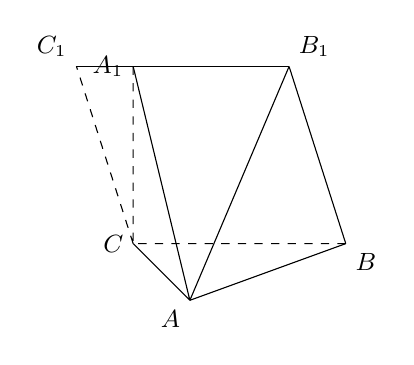
\begin{tikzpicture}[x=0.9cm,y=0.9cm,every node/.style={font=\small}]
  \coordinate (A)  at (1.8,0.2);
  \coordinate (B)  at (4,1);
  \coordinate (C)  at (1,1);
  \coordinate (A1) at (1,3.5);
  \coordinate (B1) at (3.2,3.5);
  \coordinate (C1) at (0.2,3.5);

  % 棱柱可见棱、遮挡棱，以及原图中标出的 A_1C 与 AB_1
  \draw (A)--(B) (A)--(C) (A)--(A1);
  \draw (A1)--(B1) (B1)--(C1) (C1)--(A1);
  \draw (B)--(B1) (A)--(B1);
  \draw[dashed] (B)--(C) (C)--(C1) (A1)--(C);

  \node[below left] at (A) {$A$};
  \node[below right] at (B) {$B$};
  \node[left] at (C) {$C$};
  \node[left] at (A1) {$A_1$};
  \node[above right] at (B1) {$B_1$};
  \node[above left] at (C1) {$C_1$};
\end{tikzpicture}
\end{center}
\nopagebreak[4]
  (1) 证明：$A_1C=AC$；

  (2) 已知 $AA_1$ 与 $BB_1$ 的距离为 $2$，求 $AB_1$ 与平面 $BCC_1B_1$ 所成角的正弦值。

\Needspace{4\baselineskip}
\textbf{解析}

\gksubpart{(1) 求证两条棱长相等}

\Needspace{5\baselineskip}
令 $C=(0,0,0)$，由 $\angle ACB=90^\circ$ 取 $A=(u,0,0)$、$B=(0,v,0)$；又因 $A_1C\perp$ 平面 $ABC$，可设 $A_1=(0,0,w)$，其中 $u,w>0$。平移向量

\nopagebreak[4]
\[
\overrightarrow{AA_1}=(-u,0,w),\qquad u^2+w^2=AA_1^2=4.
\]

\Needspace{5\baselineskip}
平面 $BCC_1B_1$ 由方向向量 $(0,v,0)$ 和 $(-u,0,w)$ 张成，其法向量可取 $(w,0,u)$。点 $A_1$ 到该平面的距离为

\nopagebreak[4]
\[
\frac{|(w,0,u)\cdot(0,0,w)|}{\sqrt{u^2+w^2}}
=\frac{uw}{2}=1.
\]

所以 $uw=2$。结合 $u^2+w^2=4$，有 $(u-w)^2=0$，即 $u=w=\sqrt2$。这证明 $A_1C=AC=\sqrt2$。

\gksubpart{(2) 求线面角的正弦}

\Needspace{5\baselineskip}
再设 $d=\overrightarrow{B}-\overrightarrow{A}=(-u,v,0)$。两平行直线 $AA_1$、$BB_1$ 的距离是

\nopagebreak[4]
\[
\frac{|d\times(-u,0,w)|}{|(-u,0,w)|}
=\frac{\sqrt{v^2w^2+u^2w^2+u^2v^2}}2.
\]

\Needspace{5\baselineskip}
令其等于 $2$，并代入 $u^2=w^2=2$，得到 $v^2=3$。向量

\nopagebreak[4]
\[
\overrightarrow{AB_1}=(-2u,v,w)
\]

\Needspace{5\baselineskip}
的模平方为 $4u^2+v^2+w^2=13$。侧面法向量 $(w,0,u)$ 的模为 $2$，且

\nopagebreak[4]
\[
|\overrightarrow{AB_1}\cdot(w,0,u)|
=|-2uw+uw|=uw=2.
\]

\Needspace{5\baselineskip}
线面角的正弦等于方向向量在法向量方向上的投影长度与方向向量长度之比，故所求为

\nopagebreak[4]
\[
\frac{2}{2\sqrt{13}}=\frac1{\sqrt{13}}.
\]

\gkanswer{答案（1）：见解析版}

\gkanswer{答案（2）：$\dfrac1{\sqrt{13}}$}

\end{answer}
\begin{answer}
\gksolhead{19}{}

\textbf{题目}：

一项试验旨在研究臭氧效应，试验方案如下：选 $40$ 只小白鼠，随机地将其中 $20$ 只分配到试验组，另外 $20$ 只分配到对照组，试验组的小白鼠饲养在高浓度臭氧环境，对照组的小白鼠饲养在正常环境，一段时间后统计每只小白鼠体重的增加量（单位：g）。

  (1) 设 $X$ 表示指定的两只小白鼠中分配到对照组的只数，求 $X$ 的分布列和数学期望；

  (2) 试验结果如下：

对照组的小白鼠体重的增加量从小到大排序为

$15.2\quad18.8\quad20.2\quad21.3\quad22.5\quad23.2\quad25.8\quad26.5\quad27.5\quad30.1$

$32.6\quad34.3\quad34.8\quad35.6\quad35.6\quad35.8\quad36.2\quad37.3\quad40.5\quad43.2$

试验组的小白鼠体重的增加量从小到大排序为

$7.8\quad9.2\quad11.4\quad12.4\quad13.2\quad15.5\quad16.5\quad18.0\quad18.8\quad19.2$

$19.8\quad20.2\quad21.6\quad22.8\quad23.6\quad23.9\quad25.1\quad28.2\quad32.3\quad36.5$

① 求 $40$ 只小白鼠体重的增加量的中位数 $m$，再分别统计两样本中小于 $m$ 与不小于 $m$ 的数据的个数，完成如下列联表：

\begin{center}
\begin{tabular}{ccc}
\toprule
 & $<m$ & $\geqslant m$ \\
\midrule
对照组 &  &  \\
试验组 &  &  \\
\bottomrule
\end{tabular}
\end{center}

② 根据①中的列联表，能否有 $95\%$ 的把握认为小白鼠在高浓度臭氧环境中与在正常环境中体重的增加量有差异？

\Needspace{10\baselineskip}
附：$K^2=\dfrac{n(ad-bc)^2}{(a+b)(c+d)(a+c)(b+d)}$，

\begin{center}
\begin{tabular}{cccc}
\toprule
$P(K^2\geqslant k)$ & $0.100$ & $0.050$ & $0.010$ \\
\midrule
$k$ & $2.706$ & $3.841$ & $6.635$ \\
\bottomrule
\end{tabular}
\end{center}

\Needspace{4\baselineskip}
\textbf{解析}

\Needspace{5\baselineskip}
\textbf{(1)} 指定的两只小白鼠进入对照组的只数服从超几何分布。总选法数为 $\binom{40}{2}=780$，因此

\nopagebreak[4]
\[
P(X=0)=\frac{\binom{20}{2}}{780}=\frac{19}{78},\quad
P(X=1)=\frac{20\cdot20}{780}=\frac{20}{39},\quad
P(X=2)=\frac{\binom{20}{2}}{780}=\frac{19}{78}.
\]

\Needspace{5\baselineskip}
期望为

\nopagebreak[4]
\[
E(X)=0\cdot\frac{19}{78}+1\cdot\frac{20}{39}+2\cdot\frac{19}{78}=1.
\]

\Needspace{5\baselineskip}
\textbf{(2)} 合并两组从小到大的数据后，第 $20$ 个值为 $23.2$，第 $21$ 个值为 $23.6$，所以

\nopagebreak[4]
\[
m=\frac{23.2+23.6}{2}=23.4.
\]

对照组中小于 $m$ 的有 $6$ 个、不小于 $m$ 的有 $14$ 个；试验组对应为 $14$ 个、$6$ 个。因此列联表为

\begin{center}
\begin{tabular}{crr}
\toprule
 & $<m$ & $\geqslant m$ \\
\midrule
对照组 & $6$ & $14$ \\
试验组 & $14$ & $6$ \\
\bottomrule
\end{tabular}
\end{center}

\Needspace{5\baselineskip}
代入题给统计量：

\nopagebreak[4]
\[
K^2=\frac{40(6\cdot6-14\cdot14)^2}{20\cdot20\cdot20\cdot20}=6.4.
\]

由于 $6.4>3.841$，达到 $95\%$ 的把握标准，可以认为两种环境下体重增加量有差异。

\gkanswer{答案（1）：$P(X=0)=\dfrac{19}{78},\ P(X=1)=\dfrac{20}{39},\ P(X=2)=\dfrac{19}{78};\ E(X)=1$}

\gkanswer{答案（2）：$m=23.4$；对照组 $(6,14)$、试验组 $(14,6)$；$K^2=6.4$，有 $95\%$ 的把握认为两组有差异。}

\end{answer}
\begin{answer}
\gksolhead{20}{}

\textbf{题目}：

已知直线 $x-2y+1=0$ 与抛物线 $C:y^2=2px$（$p>0$）交于 $A$，$B$ 两点，$|AB|=4\sqrt{15}$。

  (1) 求 $p$；

  (2) 设 $F$ 为 $C$ 的焦点，$M$，$N$ 为 $C$ 上两点，且 $\overrightarrow{FM}\cdot\overrightarrow{FN}=0$，求 $\triangle MFN$ 面积的最小值。

\Needspace{4\baselineskip}
\textbf{解析}

\Needspace{5\baselineskip}
\textbf{(1)} 由直线得 $x=2y-1$。代入抛物线：

\nopagebreak[4]
\[
y^2=2p(2y-1),\qquad y^2-4py+2p=0.
\]

\Needspace{5\baselineskip}
两交点纵坐标之差的绝对值为 $\sqrt{16p^2-8p}$；由于直线斜率为 $1/2$，弦长为其 $\sqrt5$ 倍。于是

\nopagebreak[4]
\[
\sqrt{5(16p^2-8p)}=4\sqrt{15},
\]

即 $2p^2-p-6=0$。取满足 $p>0$ 的根，得 $p=2$。

\Needspace{5\baselineskip}
\textbf{(2)} 当 $p=2$ 时，抛物线为 $y^2=4x$，焦点 $F=(1,0)$。参数化

\nopagebreak[4]
\[
M=(t^2,2t),\qquad N=(s^2,2s).
\]

\Needspace{5\baselineskip}
设 $u=ts$、$v=t-s$。焦半径向量点积为

\nopagebreak[4]
\[
\overrightarrow{FM}\cdot\overrightarrow{FN}
=(t^2-1)(s^2-1)+4ts
=(u+1)^2-v^2.
\]

\Needspace{5\baselineskip}
垂直条件给出 $v^2=(u+1)^2$。三角形面积为

\nopagebreak[4]
\[
\frac12\left|\det
\begin{pmatrix}
t^2-1&2t\\
s^2-1&2s
\end{pmatrix}\right|
=|v(u+1)|=(u+1)^2.
\]

\Needspace{5\baselineskip}
而 $t,s$ 为实数要求

\nopagebreak[4]
\[
(t+s)^2=(t-s)^2+4ts=(u+1)^2+4u=u^2+6u+1\geqslant0.
\]

\Needspace{5\baselineskip}
所以 $u\leqslant-3-2\sqrt2$ 或 $u\geqslant-3+2\sqrt2$。在后一范围，面积最小值在 $u=-3+2\sqrt2$ 取得，数值为

\nopagebreak[4]
\[
(-2+2\sqrt2)^2=12-8\sqrt2.
\]

边界处 $(t+s)^2=0$，可取 $s=-t$ 且 $t^2=3-2\sqrt2$，故该下界可以达到；另一范围的 $(u+1)^2$ 更大。

\gkanswer{答案（1）：$p=2$}

\gkanswer{答案（2）：$12-8\sqrt2$}

\end{answer}
\begin{answer}
\gksolhead{21}{}

\textbf{题目}：

已知函数 $f(x)=ax-\dfrac{\sin x}{\cos^3x}$，$x\in\left(0,\dfrac\pi2\right)$。

  (1) 当 $a=8$ 时，讨论 $f(x)$ 的单调性；

  (2) 若 $f(x)<\sin2x$，求 $a$ 的取值范围。

\Needspace{4\baselineskip}
\textbf{解析}

\Needspace{5\baselineskip}
记 $g(x)=\sin x/\cos^3x$。求导得

\nopagebreak[4]
\[
g'(x)=\frac{1+2\sin^2x}{\cos^4x}.
\]

\Needspace{5\baselineskip}
\textbf{(1)} 当 $a=8$ 时，

\nopagebreak[4]
\[
f'(x)=8-\frac{1+2\sin^2x}{\cos^4x}.
\]

\Needspace{5\baselineskip}
令 $t=\sin^2x\in(0,1)$，函数

\nopagebreak[4]
\[
\frac{1+2t}{(1-t)^2}
\]

严格递增；它等于 $8$ 当且仅当 $t=1/2$，即 $x=\pi/4$。因此 $f'(x)>0$ 于 $(0,\pi/4)$，$f'(x)<0$ 于 $(\pi/4,\pi/2)$，函数先增后减。

\Needspace{5\baselineskip}
\textbf{(2)} 按该函数不等式在给定定义域内对任意 $x$ 成立理解。由于 $x>0$，不等式等价于

\nopagebreak[4]
\[
a<R(x):=\frac{\sin2x+\sin x/\cos^3x}{x}.
\]

\Needspace{5\baselineskip}
令

\nopagebreak[4]
\[
G(x)=\sin2x+\frac{\sin x}{\cos^3x}-3x.
\]

\Needspace{5\baselineskip}
设 $t=\sin^2x$，则

\nopagebreak[4]
\[
G'(x)=2\cos2x+\frac{1+2\sin^2x}{\cos^4x}-3
=\frac{t^2(7-4t)}{(1-t)^2}>0
\quad(0<x<\pi/2).
\]

又 $G(0)=0$（取右极限），所以 $G(x)>0$，即 $R(x)>3$；同时 $\lim_{x\to0^+}R(x)=3$。于是所有 $x$ 上均严格小于 $R(x)$ 的参数恰为 $a\leqslant3$。

\gkanswer{答案（1）：在 $(0,\pi/4)$ 上单调递增，在 $(\pi/4,\pi/2)$ 上单调递减。}

\gkanswer{答案（2）：$a\leqslant3$}

\end{answer}
\begin{answer}
\gksolhead{22}{}

\textbf{题目}：

已知点 $P(2,1)$，直线 $l:\begin{cases}x=2+t\cos\alpha,\\y=1+t\sin\alpha,\end{cases}$（$t$ 为参数），$\alpha$ 为 $l$ 的倾斜角，$l$ 与 $x$ 轴正半轴、$y$ 轴正半轴分别交于点 $A$，$B$，且 $|PA|\cdot|PB|=4$。

  (1) 求 $\alpha$；

  (2) 以坐标原点为极点，$x$ 轴正半轴为极轴建立极坐标系，求 $l$ 的极坐标方程。

\Needspace{4\baselineskip}
\textbf{解析}

\Needspace{5\baselineskip}
\textbf{(1)} 直线需分别与两正半轴相交，故其斜率为负。设斜率为 $-q$，其中 $q>0$。过 $P(2,1)$ 的直线在 $x$ 轴、$y$ 轴上的截距分别为

\nopagebreak[4]
\[
A=\left(2+\frac1q,0\right),\qquad B=(0,1+2q).
\]

\Needspace{5\baselineskip}
于是

\nopagebreak[4]
\[
|PA|=\frac{\sqrt{1+q^2}}q,\qquad |PB|=2\sqrt{1+q^2}.
\]

条件 $|PA||PB|=4$ 化为 $q+1/q=2$，故 $q=1$。斜率为 $-1$ 的倾斜角为 $\alpha=3\pi/4$。

\Needspace{5\baselineskip}
\textbf{(2)} 直线方程为 $x+y=3$。代入 $x=\rho\cos\theta$、$y=\rho\sin\theta$，得

\nopagebreak[4]
\[
\rho(\cos\theta+\sin\theta)=3.
\]

\gkanswer{答案（1）：$\alpha=3\pi/4$}

\gkanswer{答案（2）：$\rho(\cos\theta+\sin\theta)=3$}

\end{answer}
\begin{answer}
\gksolhead{23}{}

\textbf{题目}：

设 $a>0$，函数 $f(x)=2|x-a|-a$。

  (1) 求不等式 $f(x)<x$ 的解集；

  (2) 若曲线 $y=f(x)$ 与 $x$ 轴所围成的图形的面积为 $2$，求 $a$。

\Needspace{4\baselineskip}
\textbf{解析}

\Needspace{5\baselineskip}
\textbf{(1)} 当 $x<a$ 时，$f(x)=a-2x$，不等式化为 $x>a/3$，得 $a/3<x<a$。当 $x\geqslant a$ 时，$f(x)=2x-3a$，不等式化为 $x<3a$，得 $a\leqslant x<3a$。合并解集：

\nopagebreak[4]
\[
\left(\frac a3,3a\right).
\]

\Needspace{5\baselineskip}
\textbf{(2)} 令 $f(x)=0$，得 $x=a/2$ 或 $x=3a/2$；图象顶点为 $(a,-a)$。与 $x$ 轴围成三角形的底长、高均为 $a$，故

\nopagebreak[4]
\[
\frac12a^2=2.
\]

由 $a>0$ 得 $a=2$。

\gkanswer{答案（1）：$\left(\dfrac a3,3a\right)$}

\gkanswer{答案（2）：$a=2$}

\end{answer}